\chapter{Construcciones}%
\label{cha:construcciones}
En este capítulo buscaremos topologías en base a unas aplicaciones con el objetivo de hacer a dichas aplicaciones continuas. Tras esto, daremos una caracterización de la topología construida. Por último, exploraremos las propiedades de las construcciones.

\section{Imágenes inversas}%
\label{sec:imagenes_inversas}
El objetivo de esta construcción es crear una topología que, al ser equipada en el conjunto de partida, haga la aplicación $f: (Y, ?) \rightarrow \left( X, \mathcal{T} \right)$ continua. Recordemos que, para poder cumplir con la definición de continuidad, las preimágenes de abiertos deben ser abiertos, luego cuantos más abiertos ``metamos'' en dicha topología más ``fácil'' será que las imágenes inversas caigan en abiertos.

Con dicha observación lo que se nos viene a la cabeza es tomar como topología la discreta, sin embargo, esto carece de interés: lo que realmente nos gustaría es la topología con menos abiertos posibles que haga la función continua.

\begin{defi}[Topología Imagen Inversa]
Sea $f: Y \rightarrow (X,\mathcal{T})$ una aplicación, definimos la \textbf{topología de la imagen inversa} como la topología menos fina que podemos equipar a $Y$ para que la aplicación $f$ sea continua, que es la topología:
$$
f^{-1} \mathcal{T} = \{f^{-1}U: U \in \mathcal{T}\}
$$
donde los abiertos son exactamente las preimágenes de los abiertos la topología de llegada.
\end{defi}

\begin{obs}
Tras la introducción de la sección, la topología de la definición parece la más razonable para ser candidata a menos fina posible, puesto que de ser topología (hay que probarlo) hemos ``metido'' los abiertos indispensables para la continuidad que son precisamente las imágenes inversas.
\end{obs}

\begin{prop}
Sea $f: (Y, f^{-1}\mathcal{T}) \rightarrow (X,\mathcal{T})$ donde $f^{-1}\mathcal{T}$ es la topología de la imagen inversa, entonces:
\begin{enumerate}
    \item $f^{-1}\mathcal{T}$ es topología. 
    \item $f^{-1}\mathcal{T}$ es la menos fina posible.
\end{enumerate}
\end{prop}
\begin{demo}
\begin{enumerate}
    \item Las imágenes inversas funcionan muy bien con uniones, intersecciones, etc. Por tanto, la demostración de que es topología es trivial.
    
    \item Consideremos cualquier otra topología $\mathcal{T}'$ en $Y$ que haga la función $f$ continua. Si tomamos un abierto $U \in f^{-1}\mathcal{T}$ en la topología inversa, entonces $\exists V \in \mathcal{T}: f^{-1}V = U$. Asimismo, como $f$ también es continua en $\mathcal{T}'$ sabemos que $U = f^{-1}V$ también es abierto en $\mathcal{T}'$, es decir, todo abierto en $f^{-1}\mathcal{T}$ es también abierto en $\mathcal{T}'$ y, por tanto, $f^{-1}\mathcal{T} \subset \mathcal{T}'$.
\end{enumerate}
\end{demo}

\subsection{Caracterización de la imagen inversa}
\label{sub:caracterizacion_de_la_imagen_inversa}
En muchas ocasiones, tendremos diagramas con varias aplicaciones entre varios espacios topológicos. En estas situaciones, es de utilidad tener algún teorema para poder identificar unas topologías con otras, ya que entender y manejar bien unas pueden tener buenas ``traslaciones'' en las otras. Es por ello que tiene gran utilidad el siguiente teorema de caracterización de la topología inversa en circunstancias como las descritas.

\begin{theo}[Propiedad universal de las inmersiones]
Sean $g: \left( Z, \mathcal{T}'' \right) \rightarrow \left( Y, \mathcal{T}' \right)$ y $f: \left( Y, \mathcal{T}' \right) \rightarrow \left( Z, \mathcal{T} \right)$ dos funciones entre espacios topológicos:
\begin{figure}[H]
        \centering    
            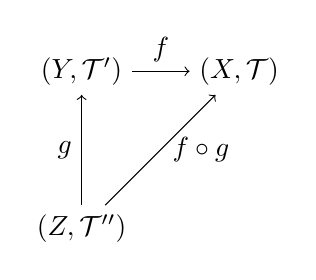
\begin{tikzpicture}[node distance=2cm, auto]
            \node(Y) {$\left( Y, \mathcal{T}' \right)$};
            \node(X) [right of=Y] {$\left( X, \mathcal{T} \right)$};
            \node(Z) [below of=Y] {$\left( Z, \mathcal{T}'' \right)$};
            \draw[->](Y) to node {$f$}(X);
            \draw[->](Z) to node [left] {$g$}(Y);
            \draw[->](Z) to node [right=0.2ex] {$f \circ g$}(X);
            \end{tikzpicture}
        \caption{\textit{Ilustración de la composición propuesta}}
        \label{prop_universal_inmersiones}
    \end{figure}
entonces $\mathcal{T}' = f^{-1}\mathcal{T}$ si y sólo si:
\[
\forall g: g \text{ cont.} \Leftrightarrow f \circ g \text{ cont.}
\]    
\end{theo}
\begin{demo}
\begin{itemize}
    \item $\Rightarrow)$ $\mathcal{T}' = f^{-1}\mathcal{T}: $ 
    \begin{itemize}
        \item $g$ cont. $\Rightarrow f \circ g$ cont. es trivial por composición de continuas.
        \item $f \circ g$ cont. $\Rightarrow g$ cont.
        
        Para probarlo, basta ver para cualquier abierto $V \in \mathcal{T}'$, $g^{-1}V$ es abierto en $\mathcal{T}''$. Por ser $\mathcal{T}'=f^{-1}\mathcal{T}$, entonces $g^{-1}V = g^{-1} f^{-1} U$ para algún abierto $U\in \mathcal{T}$, pero es que precisamente $g^{-1} f^{-1} U = \left( f \circ g \right)^{-1} U \in \mathcal{T}''$ por ser $f\circ g$ continua.
    \end{itemize}

    \item $\Leftarrow)$
	Para demostrarla vamos a ver el doble contenido de $\mathcal{T}'$ en $f^{-1}\mathcal{T} $ y viceversa.
	
	Como la propiedad de caracterización se cumple para cualquier $g$ que escojamos, podemos escoger como $g$ la aplicación identidad. De esta manera, $g \text{ cont.} \Leftrightarrow f\circ g \text{ cont.}$ implica que $id \text{ cont.} \Leftrightarrow f\circ id = f \text{ cont.}$, luego hemos demostrado que $f$ es continua.
    \begin{figure}[H]
        \centering    
            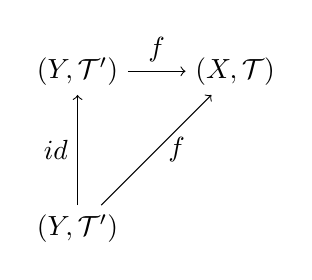
\begin{tikzpicture}[node distance=2cm, auto]
            \node(Y) {$\left( Y, \mathcal{T}' \right)$};
            \node(X) [right of=Y] {$\left( X, \mathcal{T} \right)$};
            \node(Z) [below of=Y] {$\left( Y, \mathcal{T}' \right)$};
            \draw[->](Y) to node {$f$}(X);
            \draw[->](Z) to node [left] {$id$}(Y);
            \draw[->](Z) to node [right=0.2ex] {$f$}(X);
            \end{tikzpicture}
    \end{figure}
    Y como precisamente $f^{-1}\mathcal{T}$ es la topología menos fina que posibilita la continuidad de $f$, sabemos que $\mathcal{T}' \supset f^{-1}\mathcal{T}$. 
   
   Si ahora utilizamos como $g$ la identidad puramente conjuntista (las topologías no se conservan, pero los puntos van a ellos mismos), entonces:
    \begin{figure}[H]
        \centering    
            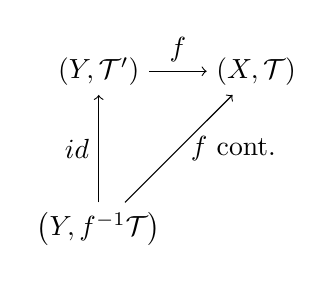
\begin{tikzpicture}[node distance=2cm, auto]
            \node(Y) {$\left( Y, \mathcal{T}' \right)$};
            \node(X) [right of=Y] {$\left( X, \mathcal{T} \right)$};
            \node(Z) [below of=Y] {$\left( Y, f^{-1}\mathcal{T} \right)$};
            \draw[->](Y) to node {$f$}(X);
            \draw[->](Z) to node [left] {$id$}(Y);
            \draw[->](Z) to node [right=0.2ex] {$f$ cont.}(X);
            \end{tikzpicture}
    \end{figure}
    de nuevo, por la propiedad de caracterización sabemos que esta nueva ``identidad'' es una función continua. Como la aplicación es entre el mismo conjunto de puntos es biyectiva, entonces cualquier abierto $U\in \mathcal{T}'$ coincide con su preimagen $f^{-1}U$. Al demostrar que la ``identidad'' es continua, entonces $\forall U \in \mathcal{T}', \ U = f^{-1}U\in f^{-1}\mathcal{T}$, es decir, que $\mathcal{T}'\subset f^{-1}\mathcal{T}$.
\end{itemize}
\end{demo}

\subsection{Inmersiones}
\label{sub:inmersiones}
La construcción anterior cobra especial relevancia cuando la aplicación $f: Y \rightarrow X$ que hemos hecho continua con la topología imagen inversa es inyectiva porque de alguna forma permite ``sumergir'' el espacio de salida en el de llegada.

\begin{defi}[Inmersión]
Sea $f:\left( Y, f^{-1}\mathcal{T} \right) \rightarrow \left( X, \mathcal{T} \right)$ una aplicación continua gracias a la topología de la imagen inversa, decimos que es una \textbf{inmersión} si y sólo si es inyectiva.
\end{defi}

\begin{prop}[Caracterización de Inmersiones]
Sea $f: \left( Y, \mathcal{T}' \right) \rightarrow \left( X, \mathcal{T} \right)$ una aplicación entre espacios topológicos, entonces:
\[
    f\text{ es inmersión} \Leftrightarrow f: \left( Y, \mathcal{T}' \right) \xrightarrow{\text{homeo.}} \left( f\left( Y \right), \mathcal{T}|_{f\left( Y \right)} \right)
\]
\end{prop}
\begin{demo}
\begin{itemize}
    \item $\Rightarrow)$ Tenemos que $f: \left( Y, f^{-1}\mathcal{T} \right) \rightarrow \left( f\left( Y \right), \mathcal{T}|_{f\left( Y \right)} \right)$. 

    Como $f$ es inmersión sabemos que es inyectiva, lo que sumado a que el espacio de llegada es $f(Y)$, nos permite saber que es sobreyectiva y, por tanto, biyectiva. De los requisitos para ver que es un homeomorfismo, bastaría con ver que es abierta y continua:
    \begin{itemize}
        \item Continua:
        
        Si escogemos un abierto cualquier $U\in \mathcal{T}\mid_{f(Y)}$, por ser abierto de la topología relativa, sabemos que $\exists W \in \mathcal{T}: U = f\left( Y \right) \cap W $ y entonces su imagen inversa
        \[
        f^{-1}\left( U \right) = f^{-1}\left( W \cap f\left( Y \right) \right) = Y \cap f^{-1}\left( W \right) = f^{-1}\left( W \right) \in f^{-1}\mathcal{T}
        \]

        \item Abierta:
        
        Observamos que cualquier abierto $U \in f^{-1}\mathcal{T}$ de la topología imagen inversa es preeimagen de un abierto de la topología de llegada, es decir, $\exists W \in \mathcal{T}: f^{-1}W = U$. Por tanto, si calculamos la imagen de $U$ por $f$, tenemos que:
        \[
        fU = ff^{-1}W = W \cap f\left( Y \right) \ab f\left( Y \right)
        \]
        es decir que $fU$ es abierto en $f\left( Y \right)$.
    \end{itemize}

    %TODO: Posiblemente mal. Algo de la relativa 
    \item $\Leftarrow)$ Veamos por el doble contenido que $\mathcal{T}' = f^{-1}\mathcal{T}$
    \begin{itemize}
        \item $\subset)$
        
        Sea $U \in \mathcal{T}'$, como es homeomorfismo es abierto, luego $fU\in \mathcal{T}|_{f\left( Y \right)}$, es decir, $\exists W \in \mathcal{T}'|_{f\left( Y \right)}: f^{-1}W = U$, luego podemos decir que $U \in f^{-1}\mathcal{T}$. 
        \item $\supset)$
        
        Sea $U \in f^{-1}\mathcal{T}$, por definición, $\exists W \in \mathcal{T}|_{f\left( Y \right)}: f^{-1}W = U$ y, como $f$ es continua en $\mathcal{T}'$, $U = f^{-1} W \in \mathcal{T}'$.
    \end{itemize}
\end{itemize} 
\end{demo}

\begin{obs}
Podemos extraer de la definición, pero sobre todo de la caracterización anterior de inmersión las siguientes conclusiones:
\begin{enumerate}
    \item Si una función $f: Y \rightarrow X$ es inyectiva, continua y abierta o cerrada, entonces es inmersión.
    \begin{demo}
    La caracterización de imagen inversa exige continuidad, biyectividad y apertura o cierre (es decir, que sea homeomorfismo) de la aplicación $g: Y \rightarrow f(Y)$. Como $f$ es inyectiva y coincide con $g$ en la imagen $f(Y)$, ésta última también es inyectiva, luego por ser sobreyectiva es biyectiva. La continuidad también se extiende a $g$ naturalmente y falta solo ver que es abierta o cerrada respectivamente. Si $f$ lo es, entonces para cualquier abierto o cerrado $W\subset Y$ su imagen $f(W)$ será abierta o cerrada en $X$. Del mismo modo, para cualquier abierto o cerrado $W\subset Y$ su imagen $g(W)$ se puede escribir como $g(W) = f(W)\cap f(Y)$ que es abierto o cerrado por ser un corte de un abierto o cerrado ambiente con el subespacio $f(Y)$.
    \end{demo}

    \item Si $f: Y \rightarrow X$ es una inmersión, entonces:
	\begin{itemize}
		\item es una aplicación abierta si y sólo si 	$f(Y)$ es abierto en $X$.
		\item es una aplicación cerrada si y sólo si $f(Y)$ es cerrado en $X$.
	\end{itemize}	    
    
    \begin{demo}
    En ambos casos, la implicación de izquierda a derecha es trivial, luego sólo es necesaria la de derecha a izquierda:
    \begin{itemize}
        \item 
        $\forall V = f^{-1}U \in f^{-1}\mathcal{T}, \ fV = \overbrace{U \cap f\left( Y \right)}^{\text{inter. abiertos}} \in \mathcal{T}$.
        \item 
        $\forall C \cerr  f^{-1}\mathcal{T}, \ Y\setminus C = f^{-1} U \in f^{-1}\mathcal{T} \Rightarrow f\left( C \right) = \underbrace{\left( X\setminus U \right) \cap f\left( Y \right)}_{\text{inter. cerrados}}  \cerr X$ 
    \end{itemize} 
    \end{demo}

    \item Las inmersiones y la apertura o cierre de la aplicación no están relacionadas. Esto quiere decir que existen inmersiones que no son abiertas ni cerradas, que sólo son abiertas, que sólo son cerradas y ambas cosas simultáneamente.
\end{enumerate}
\end{obs}

\begin{obs}
Las inmersiones son las que justifican la idea de considerar unos espacios como subespacios de otros. Las frases ``el plano proyectivo real no es un subespacio de $\mathbb{R}^3$'', ``la esfera no es un subespacio de $\mathbb{R}^2$'' o ``el plano proyectivo real es un subespacio de $\mathbb{R}^4$'' se refieren a esto mismo: cuándo hay o no hay una inmersión del primer espacio en el segundo, es decir, un subespacio del segundo homeomorfo al primero.
\end{obs}

\section{Imágenes directas}%
\label{sec:imagenes_directas}
El objetivo de esta construcción es crear una topología que, al ser equipada en el conjunto de llegada, haga la aplicación $f: (X, \mathcal{T}) \rightarrow \left( Y, ? \right)$ continua. De nuevo, recordemos que, para poder cumplir con la definición de continuidad, las preimágenes de abiertos deben ser abiertos, luego cuantos menos abiertos ``metamos'' en dicha topología menos posibilidades habrá de que sus preimágenes no caigan en abiertos.

Con dicha observación, en este caso lo que se nos viene a la cabeza es tomar como topología la trivial, sin embargo, esto vuelve a carecer de interés: lo que realmente nos gustaría es la topología con más abiertos posibles que haga la función continua.

\begin{defi}[Topología Imagen Directa]
Sea $f: (X,\mathcal{T}) \rightarrow Y$ una aplicación, definimos la \textbf{topología de la imagen directa} como la topología más fina que podemos equipar a $Y$ para que la aplicación $f$ sea continua, que es la topología:
$$
f \mathcal{T} = \{V \subset Y: f^{-1}V \in \mathcal{T}\}
$$
donde los abiertos son exactamente aquellos cuyas preimágenes son abiertos de la topología de salida.
\end{defi}

\begin{obs}
Tras la introducción de la sección, de nuevo, parece que la topología de la definición es la más razonable para ser candidata a más fina posible, puesto que de ser topología (hay que probarlo) hemos ``metido'' todo lo que podemos meter como abierto conservando el requisito de la continuidad.
\end{obs}

\begin{prop}
Sea $f: (X,\mathcal{T}) \rightarrow (Y, f\mathcal{T})$ donde $f\mathcal{T}$ es la topología de la imagen directa, entonces:
\begin{enumerate}
    \item $f\mathcal{T}$ es topología. 
    \item $f\mathcal{T}$ es la más fina posible.
\end{enumerate}
\end{prop}

\begin{demo}
\begin{enumerate}
    \item Trivial.
    \item Consideremos cualquier otra topología $\mathcal{T}'$ en $Y$ tal que haga $f$ continua. Si tomamos un abierto $U \in \mathcal{T}'$, como conserva la continuidad , $f^{-1} U = W \in \mathcal{T}$. Sin embargo, tal y como hemos definido $f \mathcal{T}$, sabemos que $U \in f \mathcal{T}$ porque $W \ab X$, luego $\mathcal{T}'\subset f\mathcal{T}$.
\end{enumerate}
\end{demo}

\subsection{Caracterización de la imagen directa}
\label{sub:caracterizacion_de_la_imagen_directa}
De nuevo, en las situaciones en las que haya diagramas con varias aplicaciones entre varios espacios topológicos, es de utilidad tener algún teorema para poder identificar unas topologías con otras, ya que entender y manejar bien unas pueden tener buenas ``traslaciones'' en las otras. Por ello, tiene gran utilidad el teorema de caracterización de la topología directa en circunstancias como las descritas.

\begin{theo}[Propiedad universal de las identificaciones]
Sean $g: \left( Y, \mathcal{T}' \right) \rightarrow \left( Z, \mathcal{T}'' \right)$ y $f: \left( X, \mathcal{T} \right) \rightarrow \left( Y, \mathcal{T}' \right)$ dos funciones entre espacio topológicos
    \begin{figure}[H]
        \centering    
            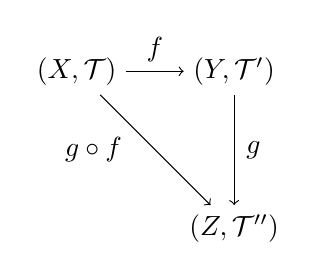
\begin{tikzpicture}[node distance=2cm, auto]
            \node(X) {$\left( X, \mathcal{T} \right)$};
            \node(Y) [right of=X] {$\left( Y, \mathcal{T}' \right)$};
            \node(Z) [below of=Y] {$\left( Z, \mathcal{T}'' \right)$};
            \draw[->](X) to node {$f$}(Y);
            \draw[->](X) to node [left=0.3cm] {$g \circ f$}(Z);
            \draw[->](Y) to node [right=0.2ex] {$g$}(Z);
            \end{tikzpicture}
        \caption{\textit{Ilustración de la composición propuesta}}
        \label{prop_universal_directas}
    \end{figure}
entonces $\mathcal{T}' = f\mathcal{T}$ si y sólo si:
	\[
        \forall g, \ g \text{ cont.} \Leftrightarrow g \circ f \text{ cont.}
	\]
\end{theo}
\begin{demo}
\begin{itemize}
    \item $\Rightarrow)$ $\mathcal{T}' = f\mathcal{T}: $ 
    \begin{itemize}
        \item $g$ cont. $\Rightarrow g \circ f$ cont. es trivial por composición de continuas.
        \item $g \circ f$ cont. $\Rightarrow g$ cont.
        
        Si escogemos un $W \in \mathcal{T}''$ sabemos que $f^{-1}\left( g^{-1} W \right) = \left( g \circ f \right)^{-1} W \in \mathcal{T}$ porque la aplicación $g\circ f$ es continua. Sin embargo, que $f^{-1} V \in \mathcal{T}$ implica que $V\in \mathcal{T}'$ porque $\mathcal{T}' = f\mathcal{T}$, luego $g^{-1}W \in \mathcal{T}'$, es decir, es continua.
    \end{itemize}

    \item $\Leftarrow)$
    Para demostrarla vamos a ver el doble contenido de $\mathcal{T}'$ en $f^{-1}\mathcal{T} $ y viceversa.
    
    Como la caracterización se cumple para cualquier $g$, en particular podemos seleccionar como $g$ la identidad. Como la identidad es continua, por la caracterización, $id \circ f = f$ es continua y, como $f\mathcal{T}$ es la topología más fina que hace $f$ continua, entonces $\mathcal{T}'\subset f\mathcal{T}$.

    \begin{figure}[H]
        \centering    
            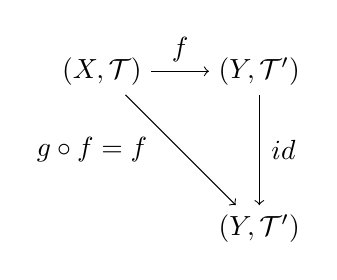
\begin{tikzpicture}[node distance=2cm, auto]
            \node(X) {$\left( X, \mathcal{T} \right)$};
            \node(Y) [right of=X] {$\left( Y, \mathcal{T}' \right)$};
            \node(Z) [below of=Y] {$\left( Y, \mathcal{T}' \right)$};
            \draw[->](X) to node {$f$}(Y);
            \draw[->](X) to node [left=0.3cm] {$g \circ f = f$}(Z);
            \draw[->](Y) to node [right=0.2ex] {$id$}(Z);
            \end{tikzpicture}
    \end{figure}
    
    De la misma manera que antes, podemos seleccionar como $g$ la identidad meramente conjuntista (donde cada punto va a sí mismo, pero no se conserva la topología porque son distintas la de salida y la de llegada). 
    \begin{figure}[H]
        \centering    
            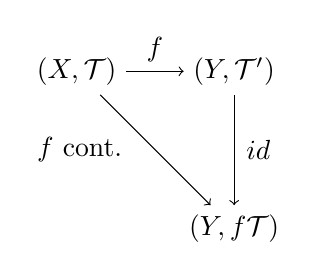
\begin{tikzpicture}[node distance=2cm, auto]
            \node(X) {$\left( X, \mathcal{T} \right)$};
            \node(Y) [right of=X] {$\left( Y, \mathcal{T}' \right)$};
            \node(Z) [below of=Y] {$\left( Y, f\mathcal{T} \right)$};
            \draw[->](X) to node {$f$}(Y);
            \draw[->](X) to node [left=0.3cm] {$f$ cont.}(Z);
            \draw[->](Y) to node [right=0.2ex] {$id$}(Z);
            \end{tikzpicture}
    \end{figure}
	En este caso, como $f$ va de $(X,\mathcal{T})$ a $(Y, f\mathcal{T})$ es continua por definición de $f\mathcal{T}$ y, por la caracterización, sabemos que la ``identidad'' que hemos seleccionado también lo es. Esto quiere decir que $\forall W \in f\mathcal{T}, id^{-1} W = W \in \mathcal{T}'$, por tanto, $f\mathcal{T}\subset \mathcal{T}'$.
\end{itemize}
\end{demo}

\begin{obs}
$f\left( X \right)$ es abierto y cerrado en $f\mathcal{T}: \begin{cases}
    \forall y \in Y \setminus f\left( X \right), f^{-1}y = \emptyset \in \mathcal{T} \Rightarrow \{y\} \in f\mathcal{T}\\
    f^{-1}f\left( X \right) = X \in \mathcal{T} \Rightarrow f\left( X \right) \in f\mathcal{T}
\end{cases}$
\end{obs}

%TODO: En sus apuntes el orden es distinto a como lo dio en clase. De momento, lo dejo como en los apuntes.
\subsection{Identificaciones}
\label{sub:identificaciones}
La construcción anterior cobra especial relevancia cuando la aplicación $f: Y \rightarrow X$ que hemos hecho continua con la topología imagen directa es sobreyectiva porque de alguna forma permite ``identificar'' el espacio de llegada en el de salida.

\begin{defi}[Identificación]
Sea $f: \left( X, \mathcal{T} \right) \rightarrow \left( Y, \mathcal{T}' \right)$ una aplicación sobreyectiva, decimos que es una \textbf{identificación} si y sólo si $\mathcal{T}' = f\mathcal{T}$.
\end{defi}

\begin{obs}
\begin{enumerate}
    \item Las identificaciones verifican $V \stackrel{\text{ab}}{\subset} Y \Leftrightarrow f^{-1}V \stackrel{\text{ab}}{\subset} X$ y la continuidad $V \stackrel{\text{ab}}{\subset } Y \Rightarrow f^{-1}V \stackrel{\text{ab}}{\subset} X$.

	\item Si una función $f: X \rightarrow Y$ es sobreyectiva, continua y abierta o cerrada, entonces es identificación.
	\begin{demo}
	Las hipótesis ya nos otorgan la continuidad y la sobreyectividad, hay que demostrar pues que $\mathcal{T}' = f\mathcal{T}$ utilizando que es abierta o cerrada.
	\begin{itemize}
		\item Abierta:
	
		Hay que ver que $\forall V \subset Y : f^{-1} V \ab X, \ V \ab Y$. Por ser $f$ sobreyectiva, $f^{-1}V$ está bien definido y, por tanto, podemos escribir $V=f(f^{-1}V)$. Como $f$ es abierta, $\forall W \ab X : f(W) \ab Y$ y como $f^{-1}V$ es abierto por la continuidad de $f$, entonces $V \ab Y$.
		
		\item Cerrada:
		
		$f^{-1}V \stackrel{\text{ab}}{\subset} X \stackrel{\text{cerr.}}{\Rightarrow} \underbrace{f \left( X \setminus f^{-1}\left( V \right) \right)}_{\stackrel{\text{sobr.}}{=} Y\setminus V}  \cerr Y \Rightarrow V \stackrel{\text{ab}}{\subset} Y$		
	\end{itemize}
	\end{demo}
	
	 \item Las identificaciones y la apertura o cierre de la aplicación no están relacionadas. Esto quiere decir que existen identificaciones que no son abiertas ni cerradas, que sólo son abiertas, que sólo son cerradas y ambas cosas simultáneamente.
\end{enumerate}
\end{obs}


\subsection{Espacio Cociente}
\label{sub:cocientes}
Para entender los abiertos de una imagen directa es conveniente representarlos en el dominio. El concepto es conjuntista en realidad:

\begin{defi}[Conjunto Saturado]
Sea $A \subset X$ un subconjunto de puntos, decimos que es \textbf{saturado respecto de $f$} si y sólo si $f^{-1}f\left( A \right) = A$.
\end{defi}

\begin{prop}[Caracterización de abiertos de $f\mathcal{T}$]
Sea $f : (X, \mathcal{T}) \rightarrow (Y, f\mathcal{T})$ donde $f\mathcal{T}$ es la topología imagen directa, los abiertos de $f\mathcal{T}$ son las imágenes de los abiertos saturados de $\mathcal{T}$, es decir:
\[
f\mathcal{T} := \{fU \mbox{ donde } U \in \mathcal{T} f^{-1}fU = U\}
\]
\end{prop}
\begin{demo}
\begin{itemize}
    %TODO: No sé si está del todo bien.
    \item $\Rightarrow)\ V \in f\mathcal{T} \Rightarrow f^{-1}V \in \mathcal{T}$ y $V \stackrel{f \text{ sobre}}{=} f^{-1}fV$, es decir, que $f^{-1} V$ es saturado.
    \item $\Leftarrow)$ Sea $V \in Y: \exists U \in \mathcal{T}$, saturado tal que: $fU = V$. Debemos ver que $f^{-1}V \in \mathcal{T}$.

    Como $f^{-1}V = f^{-1}fU \stackrel{\text{sat.}}{=} U \in \mathcal{T}$ ya lo tenemos.
\end{itemize}
\end{demo}

\begin{obs}
Los abiertos \underline{no} saturados de $X$ pueden tener imágenes \underline{no} abiertas de $Y$. 
\end{obs}

\begin{ej}
\begin{enumerate}
    %TODO: Hacer la circunferencia con todo R
    \item Consideremos la aplicación que transforma el intervalo $[0,1]$ en la circunferencia unidad de $\mathbb{R}^2$ definida como:
    \begin{align*}
        f: \left[ 0, 1 \right] &\longrightarrow \mathbb{S}^1 \\
        t &\longmapsto \left( \cos 2\pi t, \sin 2\pi t \right)
    \end{align*}
    que geométricamente es:
    \begin{figure}[H]
        \centering
        \begin{tikzpicture}
            %Flechas y texto
            \draw[gray] (0,0) -- (3,0); 
            \draw[green, ->] (0,0) -- (1,0); 
            \draw[green, ->] (3,0) -- (2,0); 
            \draw[red, ->] (3,0.4) -- (2.2,0.4); 
            \node[green] at (3.1,0.03) [right] {Saturado};
            \node[red] at (3.05,0.45) [right] {No saturado};

            %0 y 1
            \node[gray] at (0,0) [below] {$0$};
            \node[gray] at (0,0) {\textbullet};

            \node[gray] at (3,0) [below] {$1$};
            \node[gray] at (3,0) {\textbullet};

            %t saturado
            \node[gray] at (1.5,0.3) {$t$};
            \node[gray] at (1.5,0) {\textbullet};
            \node[gray] at (1.5,-0.3) {Saturado};

            %Paréntesis t
            \node[gray] at (1.3,0) {(};
            \node[gray] at (1.7,0) {)};

            \draw [gray, decorate, decoration = {brace}] (5.1,0.6) -- (5.1,-0.2);
            \node[gray] at (5.2,0.2) [right] {Abierto};

            %Función
            \node(X) at (-1,0) {$X$};
            \node(S) at (-1,-1.5) {$\mathbb{S}^1$};
            \draw[->](X) -- node [left] {$f$} (S);

            %Circulo 
            \draw[color=gray, very thick,
                decoration={markings, mark=at position 0.07 with \arrow[green]{)};,
                                      mark=at position 0.35 with \arrow{(};,
                                      mark=at position 0.47 with \arrow{)};,
                                      mark=at position 0.95 with \arrow[green]{(};,
                                      mark=at position 0.97 with \arrow[red]{(};,
                           },
                postaction={decorate}
                ] (1.5,-2) circle (1);
                %Centro
                \node(O) [gray] at (1.5,-2) {\textbullet};
                %Izquierda
                \node(izq) [gray] at (0.7,-1.4) {\textbullet};
                %Derecha
                \node(der) [gray] at (2.5,-2) {\textbullet};
                %Radio derecho
                \draw[gray, dashed] (O) -- (der);
                %Radio izquierdo
                \draw[gray, dashed] (O) -- (izq);
                
            %Entorno derecho
            \node[gray] at (der) [right] {$f\left( 0 \right) = f\left( 2 \pi \right)$};
            \node[green] at (2.5,-1.4) [right] {Es entorno abierto de $f\left( 0 \right)$};
            \node[red] at (2.5,-2.7) [right] {No es entorno abierto de $f\left( 0 \right)$};

            %Entorno izquierdo
            \node[gray] at (izq) [left] {$f\left( t \right)$};
            \draw[->, thick, gray] (-0.7,-2.3) -- (0.2,-1.8);
            \node[gray] at (0.5,-2.7) [left] {Entorno en $f \mathcal{T}$};

            %Localización
            \draw [gray, decorate, decoration = {brace}] (7.4,-1.1) -- (7.4,-3);
            \node[gray] at (7.5,-2.05) [right] {En $f\mathcal{T}$};
        \end{tikzpicture}
        \caption{\textit{La topología imagen directa es la usual en $\mathbb{S}^1$}}
        \label{fig:proyeccion_exponencial_img_directa}
    \end{figure}

    \item Tenemos:
    \begin{align*}
        f: R = \left[ 0, 1 \right] \times \left[ 0, 1 \right] &\rightarrow C \subset \mathbb{R}^3: x^2 + y^2 = 1,\ 0 \le z \le 1\\
        \left( s, t \right) &\mapsto \left( \cos 2\pi s, \sin 2\pi s, t \right) 
    .\end{align*}
    que geométricamente es:
    \begin{figure}[H]
        \centering
        \incfig[0.9]{rectángulo-a-cilindro-por-imagen-directa.}
        \caption{\textit{Analizando los abiertos saturados y no saturados se concluye que la topología imagen directa es la usual en el tronco del cilindro.}}
        \label{fig:rectángulo-a-cilindro-por-imagen-directa.}
    \end{figure}
\end{enumerate}
\end{ej}

\begin{defi}[Relación de inyectividad]
Llamamos \textbf{relación de inyectividad} a aquella relación de equivalencia que viene dada por una función $f$ tal que dos elementos están relacionados si comparten imagen:
\[
x \sim y \Leftrightarrow f\left( x \right) = f\left( y \right)
\]
\end{defi}

\begin{defi}[Proyección canónica]
Llamamos \textbf{proyección canónica} respecto de una relación de equivalencia a la aplicación:
\begin{align*}
    p: X &\rightarrow \faktor{X}{\sim}\\ 
    x &\mapsto \left[ x \right]
\end{align*}
donde $\left[ x \right]$ es la clase de equivalencia de $x$.
\end{defi}
Con esto vemos que dentro de las identificaciones tenemos el caso particular del cociente:
\[
p: \left( X, \mathcal{T} \right) \rightarrow \faktor{X}{\sim}.
\]
Con esto definimos:
\begin{defi}[Topología cociente]
Llamamos \textbf{topología cociente} a: 
\[
    \faktor{\mathcal{T}}{\sim} := \left\{ U \subset \faktor{X}{\sim}: p ^{-1}\left( U \right) \in \mathcal{T} \right\}
\]
que viene a ser la topología imagen directa por $p$.
\end{defi}

\begin{figure}[H]
    \centering    
        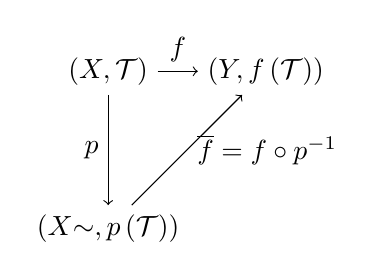
\begin{tikzpicture}[node distance=2cm, auto]
        \node(X) {$\left( X, \mathcal{T} \right)$};
        \node(Y) [right of=X] {$\left( Y, f\left( \mathcal{T} \right) \right)$};
        \node(Z) [below of=X] {$\left( \faktor{X}{\sim}, p\left( \mathcal{T} \right) \right)$};
        \draw[->](X) to node {$f$}(Y);
        \draw[->](X) to node [left] {$p$}(Z);
        \draw[->](Z) to node [right=0.2] {$\overline{f} = f \circ p^{-1}$}(Y);
        \end{tikzpicture}  
        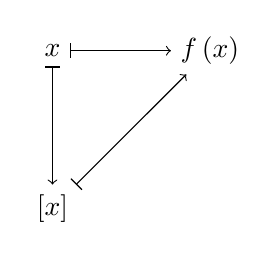
\begin{tikzpicture}[node distance=2cm, auto]
        \node(x) {$x$};
        \node(y) [right of=x] {$f\left( x \right)$};
        \node(z) [below of=x] {$\left[ x \right]$};
        \draw[|->](x) to (y);
        \draw[|->](x) to (z);
        \draw[|->](z) to (y);
        \end{tikzpicture}
        \caption{\textit{Representación de la composición del cociente}}
\end{figure}

\begin{obs}
La relación de equivalencia que vamos a usar es la que viene dada por la relación de \underline{inyectividad} respecto de $f$. Por esta razón, $\overline{f}$ será una biyección.
\end{obs}
\begin{demo}
Sea $z \in Y$ como $f$ es suprayectiva $\exists x \in X: f\left( x \right) = z$. A su vez, $y \in \left[ x \right] \Leftrightarrow f\left( x \right) = f\left( y \right) \Rightarrow \overline{f}\left( \left[ x \right] \right) = z$. Con esto, $\overline{f}$ es sobreyectiva y bien definida.

Sean ahora $\left[ x \right], \left[ y \right] \in \faktor{X}{\sim}$ tal que $\overline{f}\left[ x \right] = \overline{f}\left[ y \right] \Rightarrow f\left( x \right) = f\left( y \right) \Rightarrow \left[ x \right] = \left[ y \right]$. Por tanto, también es inyectiva.
\end{demo}

%TODO: No estoy seguro de como es esta proposición
\begin{prop}
\begin{enumerate}
    \item $\exists \overline{f} \Leftrightarrow x \sim y \Rightarrow f\left( x \right) \sim f\left( y \right)$
    \item $\exists \overline{f} : \overline{f}$ continua $\Leftrightarrow f$ continua.
    \item $\exists \overline{f}: \overline{f} \begin{cases}
        \text{sobre. }\\ 
        \text{iny. 1-1}\\ 
    \end{cases} \Leftrightarrow f \begin{cases}
        \text{sobre.}\\ 
        x \sim y \Leftarrow f \left( x \right) \sim f \left( y \right)
    \end{cases}$

    \item $\overline{f}$ homeomorfa $\Leftrightarrow f$ identificación.
    %TODO: Fix 
    \begin{figure}[H]
        \centering
        \begin{tikzpicture}[node distance=2cm, auto]
        \node(X) {$\left( X, \mathcal{T} \right)$};
        \node(Y) [right=2cm of X] {$\left( Y, \mathcal{T}' \right)$};
        \node(Z) [below=1.5cm of X] {$\left( \faktor{X}{\sim}, \overline{\mathcal{T}} \right)$};
        \draw[->](X) to node {$f$} node [below] {ident.}(Y);
        \draw[->](X) to node [left] {$p$} (Z);
        \draw[->](Z) to node [left=0.2] {$\overline{f}$} node [below=0.3] {homeo.} (Y);
        \end{tikzpicture}  
        \caption{\textit{Relación entre el cociente y una identificación.}}
        \label{fig:relacion_cociente_identificacion}
    \end{figure}
\end{enumerate} 
\end{prop}
\begin{demo}
\begin{enumerate}
    \item Por la definición de $\sim$ y de $\overline{f}$.
    %TODO: Corregir. Creo que se puede usar la propiedad universal
    \item Sea $\overline{f}$ continua. Tomemos $U \in \mathcal{T}' \Rightarrow \overline{f}^{-1}U \in \overline{\mathcal{T}}$. Como $p$ es continua por definición de $\overline{\mathcal{T}}$, $f^{-1} U = p^{-1} \overline{f}^{-1} U \in \mathcal{T}$. Por lo que $f$ es continua.

    Sea ahora $f$ continua. Tomemos $U \in \mathcal{T}' \Rightarrow W = f^{-1}U \in \mathcal{T}$. Al ser $p$ sobreyectiva $W = p^{-1}pW$, es decir, que $pW \in \overline{\mathcal{T}}$ (ya que $p^{-1}\left( p W \right) \in \mathcal{T}$ y la definición de $\overline{\mathcal{T}}$).

    \item (Anterior observación) Si $\overline{f}$ es inyectiva 1-1 $\Rightarrow \underbrace{\overline{f}\left[ x \right] = \overline{f}\left[ y \right]}_{\Leftrightarrow f\left( x \right) \sim f\left( y \right)} \Rightarrow \underbrace{\left[ x \right] = \left[ y \right]}_{\Leftrightarrow x \sim y}$
\end{enumerate}
\end{demo}

\begin{pg}
    Los cocientes son cómodos para definir espacios, las identificaciones son mejores para estudiar las propiedades que tenemos. Conviene pues tener triángulos como el anterior (\ref{fig:relacion_cociente_identificacion}). 

    Se puede contemplar $Y$ como un modelo del cociente. Es decir, utilizamos la identificación como ``modelo teórico'' y el cociente como ``modelo geométrico''. Esto no siempre será posible ya que dependerá de ciertas propiedades geométricas que veremos.
\end{pg}

\begin{ej}[Anteriores]
\begin{itemize}
    \item Circunferencia y el cilindro como cocientes:
    \begin{figure}[H]
        \centering
        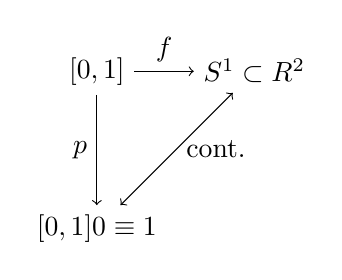
\begin{tikzpicture}[node distance=2cm, auto]
            \node(X) {$\left[ 0, 1 \right]$};
            \node(Y) [right of=X] {$\mathbb{S}^1 \subset \mathbb{R}^2$};
            \node(Z) [below of=X] {$\faktor{\left[ 0, 1 \right]}{0 \equiv 1}$};
            \draw[->](X) to node {$f$} (Y);
            \draw[->](X) to node [left] {$p$} (Z);
            \draw[<->](Z) to node [right] {cont.}(Y);
        \end{tikzpicture}
        %TODO: arreglar distancia X a Y
        \begin{tikzpicture}[node distance=2cm, auto]
            \node(X) {$\left[ 0, 1 \right] \times \left[ 0, 1 \right]$};
            \node(Y) [right=1.5cm of X] {$C \subset \mathbb{R}^3$};
            \node(Z) [below of=X] {$\faktor{\left[ 0, 1 \right] \times \left[ 0, 1 \right]}{\left( 0, t \right) \equiv \left( 1, t \right)}$};
            \draw[->](X) to (Y);
            \draw[->](X) to (Z);
            \draw[<->](Z) to (Y);
        \end{tikzpicture}
        \caption{\textit{En el primero tomamos un segmento de longitud $1$ y ``pegamos'' los extremos, lo que nos da una figura equivalente a un circunferencia. En el segundo, tomamos un rectángulo de área $1$ y ``pegamos'' el lado izquierdo con el derecho directamente.}}
    \end{figure}

    Para la circunferencia tenemos:
    \[
        \faktor{X}{\sim} = \left\{ \left\{ t \right\} : 0 < t < 1, \left\{ 0, 1 \right\} \right\}
    \]
    %TODO: Posiblemente mal
    la biyección entre el cociente y la esfera se da por el punto (3) de la anterior proposición y la continuidad por (2). Por último, la identificación se da por el anterior ejemplo.

    \item Para representar cocientes se utilizan dibujos que indican las identificaciones en los espacios de partida:
    \begin{figure}[H]
        \centering
        \hspace{2cm}
        \begin{tikzpicture}
            \node at (1,2.3) {Cilindro};
            \filldraw[color=cyan, fill=cyan!5, very thick,
                decoration={markings, mark=at position 0.18 with \arrow{>};,
                                      mark=at position 0.59 with \arrow{<};,
                           },
                postaction={decorate}
                ] (0,0) rectangle (2,2);
            \node[cyan] at (0,1.35) {\textbullet};
            \node[cyan] at (2,1.35) {\textbullet};
            \node[gray] at (2.1,1) [right] {$\left( 0, t \right) \equiv \left( 1, t \right)$};
        \end{tikzpicture}
        \begin{tikzpicture}
            \node at (1,2.3) {Banda de Möbius};
            \filldraw[color=cyan, fill=cyan!5, very thick,
                decoration={markings, mark=at position 0.18 with \arrow{>};,
                                      mark=at position 0.67 with \arrow{>};,
                           },
                postaction={decorate}
                ] (0,0) rectangle (2,2);
            \node[cyan](izq) at (0,1.35) {\textbullet};
            \node[cyan](der) at (2,0.67) {\textbullet};
            \node[cyan](O) at (1,1) {\textbullet};
            \draw[-, cyan, dashed] (izq) -- (der);
            \node[gray] at (2.1,1) [right] {$\left( 0, t \right) \equiv \left( 0, 1-t \right)$};
        \end{tikzpicture}
    \end{figure}
\end{itemize}
\end{ej}


\section{Productos (finitos)}%
\label{sec:productos_finitos_}
Supongamos que tenemos $p_i: X_1 \times \ldots X_r = Y \rightarrow \left( X_i, \mathcal{T}_i \right), 1 \le i \le r$ y buscamos hacerlas continuas. Trivialmente, podemos hacer que la topología en $X_i$ sea la discreta, sin embargo, esto carece de interés. Por esta razón, buscamos las topologías \underline{menos finas} que hagan $p_i$ continuas. 

Que $p_i$ sea continua quiere decir que $\forall U_i \in \mathcal{T}_i : p^{-1}U_i = X_1 \times \ldots U_i \times \ldots \times X_r$ debe ser abierto, es decir, que todos lo sean. Por tanto, $\bigcap_{i=1}^{r} p_i^{-1}U_i = U_1 \times \ldots \times U_r$ debe ser abierto, pero no es topología (la unión de productos no tiene porque ser producto). Por tanto, definimos:
\begin{defi}
Llamamos \textbf{topología producto}, $\mathcal{T}_1 \times \ldots \times \mathcal{T}_r$, a aquella que viene determinada por la siguiente base:
\[
\mathcal{B} = \left\{ U_1 \times \ldots \times U_r: U_i \in \mathcal{T}_i \right\}
\]
\end{defi}

\begin{ej}
La $\mathcal{T}_u$ en $\mathbb{R}^n$ es el producto de la usual en cada factor $\mathbb{R}$ de $\mathbb{R}^n$. La base de la definición de topología producto está formada por las ``bolas cuadradas'', que son productos de intervalos.
\end{ej}

\begin{theo}[Propiedad universal de la topología producto]
Sea $g: \left( Z, \mathcal{T}'' \right) \rightarrow \left( Y, \mathcal{T}' \right)$ y $p_i: \left( Y, \mathcal{T}' \right) \rightarrow \left( X_i, \mathcal{T}_i \right)$. Entonces:
    \[
    \mathcal{T}' = \prod_{i} \mathcal{T} \Leftrightarrow  
    \]
    \begin{equation}\label{eq:prop_universal_prod}
        \forall g \left[ g \text{ cont.} \Leftrightarrow \forall g_i \text{ cont.} \right]
    \end{equation}

    \begin{figure}[H]
        \centering    
            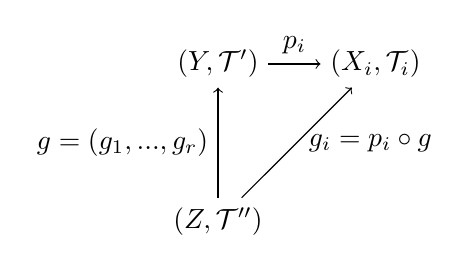
\begin{tikzpicture}[node distance=2cm, auto]
            \node(Y) {$\left( Y, \mathcal{T}' \right)$};
            \node(X) [right of=Y] {$\left( X_i, \mathcal{T}_i \right)$};
            \node(Z) [below of=Y] {$\left( Z, \mathcal{T}'' \right)$};
            \draw[->](Y) to node {$p_i$}(X);
            \draw[->](Z) to node [left] {$g = \left( g_1, ..., g_r \right)$}(Y);
            \draw[->](Z) to node [right=0.2ex] {$g_i = p_i \circ g$}(X);
            \end{tikzpicture}
        \caption{\textit{Ilustración de la composición propuesta}}
        \label{prop_universal_prod_finitos}
    \end{figure}
\end{theo}
\begin{demo}
\begin{enumerate}
    \item $\mathcal{T}' = \prod_{i} \mathcal{T}: $ 
    \begin{itemize}
        \item $g$ cont. $\Rightarrow g_i$ cont. (Todas sus componentes son continuas o composición de continuas)
        \item $g_i$ cont. $\Rightarrow g^{-1}\left( U_1 \times \ldots \times U_r \right) = \underbrace{g_1^{-1}\left( U_1 \right)}_{\mathcal{T}''} \cap \ldots \cap \underbrace{g_r^{-1}\left( U_i \right)}_{\mathcal{T}''} \in \mathcal{T}''$. (Intersección finita de abiertos) 
    \end{itemize}

    \item Por otro lado, veamos la unicidad:

    \begin{figure}[H]
        \centering    
            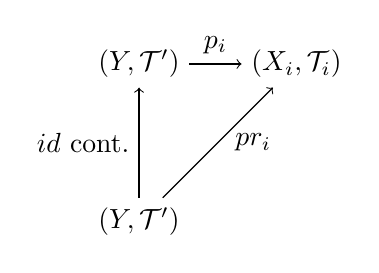
\begin{tikzpicture}[node distance=2cm, auto]
            \node(Y) {$\left( Y, \mathcal{T}' \right)$};
            \node(X) [right of=Y] {$\left( X_i, \mathcal{T}_i \right)$};
            \node(Z) [below of=Y] {$\left( Y, \mathcal{T}' \right)$};
            \draw[->](Y) to node {$p_i$}(X);
            \draw[->](Z) to node [right=0.1cm] {$pr_i$}(X);
            \draw[->](Z) to node [left] {$id$ cont.}(Y);
            \end{tikzpicture}
    \end{figure}
    Como $id$ será continua, aplicamos \ref{eq:prop_universal_prod} y tenemos que $g \circ p_i = pr_i$ es continua. Al ser $\prod_{i} \mathcal{T}_i $ la menos fina $\Rightarrow \mathcal{T}' \supset \prod_{i} \mathcal{T}_i$.

    \begin{figure}[H]
        \centering    
            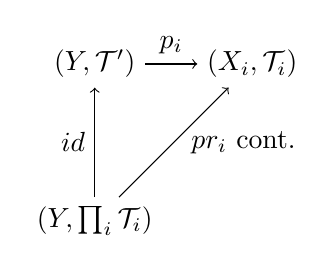
\begin{tikzpicture}[node distance=2cm, auto]
            \node(Y) {$\left( Y, \mathcal{T}' \right)$};
            \node(X) [right of=Y] {$\left( X_i, \mathcal{T}_i \right)$};
            \node(Z) [below of=Y] {$\left( Y, \prod_{i} \mathcal{T}_i \right)$};
            \draw[->](Y) to node {$p_i$}(X);
            \draw[->](Z) to node [right=0.1cm] {$pr_i$ cont.}(X);
            \draw[->](Z) to node [left] {$id$}(Y);
            \end{tikzpicture}
    \end{figure}
    Como $pr_i$ es continua por definición de $\prod_{i} \mathcal{T}_i$, aplicamos \ref{eq:prop_universal_prod} y tenemos que esta $id$ es continua. Por esta razón, $\prod_{i=1} \mathcal{T}_i \supset \mathcal{T}'$.
\end{enumerate}
\end{demo}

\begin{enun}
Demostrar (ii) sin usar que $\prod_{i} \mathcal{T}_i$ es la menos fina (usar que cumple la caracterización)
\end{enun}

%TODO: Hacer bien
\begin{ej}
La $\mathcal{T}_{\text{rad}}$ no es producto.
\begin{demo}
    Tomamos un abierto y veamos que no es producto. 
    %TODO: Dibujo

    Supongamos que sí:
    $U = \mathbb{R}^2 \setminus $ arco $\ni \left( 0, 0 \right) \Rightarrow U_1 \times U_2 \subset U$ y $\left( 0, 0 \right) \in U_1 \times U_2 \subset \mathcal{T}_{\text{rad}}$. Tomando $x_1 \in U_1$ y vemos $x = x_1 \cap r$ con $r$ línea vertical por $x_1$ con esto $y_1 = x \cap l$ con $l$ línea horizontal por $x$ no pertenece a $U$ (de lo contrario el producto $y_1$ con $x_1 = x$ pertenecería). Por tanto, $I_k = \left[ \left( 0, y_k \right), \left( x_k, y_k \right) \right]$ no tiene ningún punto en $U_1 \times U_2$. Haciendo converger $I_k$ hacía $0$ para cualquier recta por $0$ tendremos un $I_k$ que tenga intersección con la recta, es decir, la recta tendrá un punto que no pertenezca al abierto y $U$ no sería abierto ¡!

    Con esto, $\nexists x_k \rightarrow 0 \Rightarrow$ habrá un intervalo $\left( 0, \varepsilon \right)$ en el eje $x$ que no pertenece a $U_1$ y tendremos un ``vacío'' que de nuevo incumple que $U$ es abierto.
\end{demo}
\end{ej}

\begin{prop}
\begin{enumerate}
    \item $p_i: Y \rightarrow X_i$ es abierta. 
    \item $X_j \xrightarrow{\alpha_j} Y: x_j \mapsto \left( a_1, \ldots, x_j, \ldots, a_r \right)$ es inmersión ($a_i \in X_i$ fijados). La llamamos \textbf{aplicación parcial}.
\end{enumerate}
\end{prop}
\begin{demo}
\begin{enumerate}
    \item Nos vale con probarlo para una base: $p_i\left( U_1 \times \ldots \times U_r \right) = U_i$ 
    \item Trivialmente es inyectiva y continua. Por último, $X_i \rightarrow j\left( X_i \right)$ es homeomorfismo, es decir, es abierta porque:
    \[
    \begin{cases}
        \alpha_j\left( X_j \right) = \{a_1\} \times \ldots \times X_j \times \ldots \times \{a_r\} \\
        \alpha_j\left( U_j \right) = \{a_1\} \times \ldots \times U_j \times \ldots \times \{a_r\} = \alpha_j\left( X_j \right) \cap \left( X_1 \times \ldots \times U_j \times \ldots \times X_r \right) 
    \end{cases}
    \]
    que es abierto porque estamos restringiendo la topología producto a $\left\{ a_1 \right\} \times \ldots \times X_i \times \ldots \times \left\{ a_r \right\} = \alpha_j\left( X_j \right)$.
\end{enumerate}
\end{demo}

\begin{ej}
El ejemplo ahora de $\mathcal{T}_{\text{rad}}$ simplemente es porque si fuese producto sus elementos deberían ser la usual y el producto de usuales es usual que es distinta de la radial.
\end{ej}

\begin{pg}
En una topología producto todo ``se genera en productos''.
\begin{ej}
\begin{itemize}
    \item Bases de entornos: $\mathcal{V}^a = \mathcal{V}^{a_1} \times \ldots \times \mathcal{V}^{a_r} \stackrel{mut??}{=} \{V_1 \times \ldots \times V_r: V_i \in \mathcal{V}^{a_i}\} \left( a \in Y \right)$.
    \item Base de abiertos: $\mathcal{B} = \mathcal{B}_1 \times \ldots \times \mathcal{B}_r = \{B_1 \times \ldots \times B_r: B_i \in \mathcal{B}_i\}$ (esto repite la construcción de $\prod_{i} \mathcal{T}_i$)
\end{itemize}
\end{ej}
\end{pg}


%TODO: Cambiar e_i por j_i?
\section{Sumas (finitas)}%
\label{sec:sumas_finitas}
Supongamos que tenemos $e_i: \left( X_i, \mathcal{T}_i \right) \rightarrow Y = X_1 + \ldots + X_r = \left( X_1 \times \left\{ 1 \right\} \right) \cup \ldots \cup \left( X_r \times \left\{ r \right\} \right), 1 \le i \le r: x_i \mapsto \left( x_i, i \right)$ (ponemos los índices para hacerlos disjuntos) y buscamos hacerlas continuas. Trivialmente, podemos hacer que la topología en $Y$ sea la trivial, sin embargo, esto carece de interés. Por esta razón, buscamos la topología \underline{más fina} que haga $f$ continua.

Debido a que, $\forall U_i \in \mathcal{T}_i,\ e_i^{-1}\left( U_i \times \left\{ i \right\} \right)$ debe ser abierto, podemos definir lo siguiente:
\begin{defi}
Llamamos \textbf{topología suma}, $\sum_{i=1}^{k} \mathcal{T}_i$, a aquella que viene determinada por la siguiente base:
\[
\mathcal{B} = \left\{ U_1 \times \left\{ 1 \right\}, \ldots, U_r \times \left\{ r \right\}: U_i \in \mathcal{T}_i, 1 \le i \le r \right\}
\]
\end{defi}

\begin{obs}
Tenemos que los $\left\{ i \right\} \times X_i \in \sum_{i=1}^{r} \mathcal{T}_i$ son sumandos abiertos y cerrados (porque el complementario es la intersección del resto de sumandos que son abiertos?).
\end{obs}

\begin{prop}
Con la anterior definición sabemos que 
\[
e_i: \left( X_i, \mathcal{T}_i \right) \rightarrow \left( X_i\times \{i\}, \mathcal{T}|_{X_i \times \{i\}} \right),\ \forall i \in \left\{ 1, \ldots, r \right\}
\]
es inmersión abierta y cerrada.
\end{prop}
\begin{demo}
\begin{itemize}
    \item Inmersión abierta: $e_i\left( U_i \right) = U_i \times \{i\} \in \mathcal{T}$
    \item Cerrada: $Y\setminus e_i\left( X_i \right) = Y \setminus X_i \times \{i\} = \bigcup_{j \neq i} X_j \times \{j\} \in \mathcal{T}$
\end{itemize}
\end{demo}

%TODO: Fix teorema
\begin{theo}[Caracterización topología suma]
Sea $g: \left( Y, \mathcal{T}' \right) \rightarrow \left( Z, \mathcal{T}'' \right)$ y $e_i: \left( X_i, \mathcal{T}_i \right) \rightarrow \left( Y, \mathcal{T}' \right)$. Entonces:
    \[
    \mathcal{T}' = \mathcal{T}_1 + \ldots + \mathcal{T}_r \Leftrightarrow  
    \]
    \begin{equation}\label{eq:prop_universal_sum}
        \forall g \left[ g \text{ cont.} \Leftrightarrow \forall g_i \text{ cont.} \right]
    \end{equation}

    \begin{figure}[H]
        \centering    
            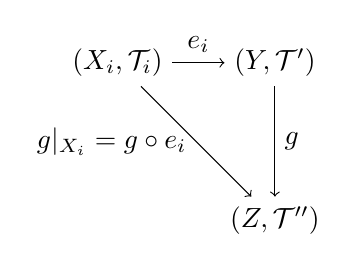
\begin{tikzpicture}[node distance=2cm, auto]
            \node(X) {$\left( X_i, \mathcal{T}_i \right)$};
            \node(Y) [right of=X] {$\left( Y, \mathcal{T}' \right)$};
            \node(Z) [below of=Y] {$\left( Z, \mathcal{T}'' \right)$};
            \draw[->](X) to node {$e_i$}(Y);
            \draw[->](X) to node [left] {$g|_{X_i} = g \circ e_i$}(Z);
            \draw[->](Y) to node {$g$}(Z);
            \end{tikzpicture}
        \caption{\textit{Ilustración de la composición propuesta}}
        \label{prop_universal_sum_finitas}
    \end{figure}
\end{theo}
%TODO: Tal vez hacerlo bien?
\begin{demo}
    Análoga a las anteriores construcciones.
\end{demo}

\begin{pg}
Localmente $Y = X_1 + \ldots + X_r$ es como sea cada $X_i$. Por ejemplo, las bases de entornos de $Y$ son las de los sumandos. Globalmente, se trata cada sumando separadamente. Por ejemplo, las bases de abiertos de los sumandos se unen para dar una base de abiertos de $Y$. Olvidando el tecnicismo $X_i \times \{i\} \equiv X_i$:
\begin{center}
   $Y$ es unión disjunta de los sumandos\\
   Los sumando son subespacios abiertos y cerrados de $Y$
\end{center}
Es un formalismo para hacer cómodamente otras construcciones. Por ejemplo, ``pegar dos discos por sus bordes'' sería:
\begin{gather*}
    \text{Disco } D \subset \mathbb{R}^2: x^2 + y^2 \le 1, \text{ borde } \partial D = \mathbb{S}^1: x^2 + y^2 = 1\\
    %TODO: Fix cociente
    \faktor{D_1 + D_2}{\sim} \quad \overbrace{\left( p, 1 \right)}^{\in \partial D} \sim \left( p, 2 \right) 
.\end{gather*}

\begin{figure}[H]
    \centering
    \incfig{dos-discos.}
    \caption{\textit{Dos discos}}
    \label{fig:dos-discos.}
\end{figure}
y más elaborado $h: \partial D \stackrel{\text{homeo.}}{\approx} \partial D$ con $\overbrace{p}^{\in \partial D} \sim h\left( p \right)$.

Finalmente, hay otros conceptos de ``suma'' más significativos que veremos en algún ejemplo.
\end{pg}


\section{Espacios proyectivos reales}%
\label{sec:espacios_proyectivos_reales}
\subsection{Geometría lineal}
\label{sub:geometría_lineal}
En primer lugar, veamos un repaso de lo visto en geometría lineal sobre espacios proyectivos.
\begin{defi}[Espacio proyectivo real]    
Usando $\sim$, proporcionalidad: 
\[
\mathbb{R}P^n = \mathbb{P}^{n} = \faktor{\mathbb{R}^{n+1}\setminus \{0\}}{\sim} \Rightarrow \mathbb{P}^{n} = \{\text{rectas vectoriales de } \mathbb{R}^{n+1}\}     
\]
Que en coordenadas es:
\begin{align*}
    \pi: \mathbb{R}^{n+1} \setminus \{0\} &\rightarrow \mathbb{P}^{n}\\
    \left( x_0, \ldots, x_n \right) &\mapsto \left( x_0 : \ldots : x_n \right) 
.\end{align*}
\end{defi}
\begin{obs}
Las ecuaciones serán de la forma: $h\in \mathbb{R}\left[ x_0, \ldots, x_n \right]$ homogénea $\Rightarrow \begin{cases}
    h\left( x \right) = 0\\
    h\left( x \right) \neq 0
\end{cases}$ está bien definido en $\mathbb{P}^{n}$.
Sabemos que el grado de la ecuación homogénea $h$ nos dará lugar a:
\begin{itemize}
    \item Grado \underline{1}: Variedades proyectivas lineales.
    \item Grado \underline{2}: Cuádricas proyectivas.
    \item Grado \underline{arbitrario}: Variedades proyectivas algebraicas.
\end{itemize}
\end{obs}

\begin{defi}[Cartas afines]
Sea $H \subset \mathbb{P}^n$ un hiperplano proyectivo. Entonces, tenemos un hiperplano lineal $\hat{H} \subset \mathbb{R}^{n+1}$, con una forma lineal asociada $h = 0$, de la siguiente forma:
\[
H = \faktor{\hat{H}\setminus \left\{ 0 \right\}}{\sim}
\]
Decimos que $H$ es \textbf{hiperplano del infinito} de la \textbf{carta afín} $U = \mathbb{P}^n \setminus H$.
\end{defi}
\begin{prop}
La aplicación 
\[
\pi|: \underbrace{\left\{ h = 1 \right\}\subset \mathbb{R}^{n+1} \setminus \left\{ 0 \right\}}_{\text{Hiperplano afín}} \rightarrow \underbrace{\mathbb{P}^{n} \setminus H}_{\left\{ h \neq 0 \right\}} = U
\]
es una biyección.
\end{prop}

\subsection{Topología de espacio proyectivos}
\label{sub:topología_de_espacio_proyectivos}
Para la topología en $U$ usaremos la imagen directa de la usual en $\left\{ h = 1 \right\} \subset \mathbb{R}^{n+1}$
\begin{prop}
Con la anterior suposición tenemos que la aplicación:
\[
\pi|: \{h = 1\} \rightarrow U
\]
es un \underline{homeomorfismo}.     
\end{prop}
\begin{demo}
Ya sabemos que es biyección por lo que queda ver que es continua y abierta/cerrada. Continua lo será por tener $U$ la topología imagen directa. Y abierta porque???%TODO
\end{demo}
%TODO: Creo que esta demostración no es de esto.
%\begin{demo}
%Veamos lo que tenemos:
%\begin{figure}[H]
%    \centering
%        \begin{tikzpicture}[node distance=2cm, auto]
%        \node(X) {$\mathbb{R}^{n+1} \setminus \left\{ 0 \right\}$ usual};
%        \node(Z) [below of=X] {$U \subset \mathbb{P}^n$ cociente};
%        \node(Y) [left=1.2cm of Z] {$\mathbb{R}^{n+1} \supset \left\{ h = 1 \right\}$};
%        \draw[->](X) to node [left] {$\pi$}(Z);
%        \draw[->](Y) to node [below] {homeo.}(Z);
%        \end{tikzpicture}
%    \captionsetup{font={color=gray}}
%    \caption[gray]{\textit{Composición propuesta}}
%    \label{}
%\end{figure}
%Tomemos $W \subset U \begin{cases}
%    \text{cociente: } \pi^{-1} \left( W \right) \ab \mathbb{R}^{n+1} \setminus \left\{ 0 \right\}\\
%    \text{homeo: } \pi^{-1}\left( W \right) \cap \left\{ h = 1 \right\} \ab \left\{ h=1 \right\}
%\end{cases}$.    
%Cociente $\Rightarrow$ homeomorfismo es trivial y significa que $\pi|_{\left\{ h=1 \right\}}$ es continua. Homeomorfismo $\Rightarrow$ cociente porque:
%\[
%\pi^{-1}\left( W \right) = \text{cono de } \underbrace{\pi^{-1}\left( W \right) \cap \left\{ h = 1 \right\}}_{A}
%\]
%Como $\left\{ h=1 \right\} \supset A$ abierto $\Leftrightarrow \text{cono}\left( A \right) \ab \mathbb{R}^{n+1} \setminus \left\{ 0 \right\}$ donde cono$\left( A \right) = \left\{ \lambda a: a \in A, \lambda \in \mathbb{R} \setminus \left\{ 0 \right\} \right\}$
%\end{demo}

\begin{prop}
La siguiente definición es topología en $\mathbb{P}^n$:
\[
W \text{ abierto si } W \cap U \text{ es abierto } \forall U \text{ carta afín.}
\]
\end{prop}
\begin{demo}
%TODO
Ni idea
\end{demo}

%TODO: Fix topologia
\begin{prop}[Topología en Pn]    
\begin{itemize}
    \item \underline{Cociente} de la usual vía $\mathbb{R}^{n+1}\setminus \{0\} \xrightarrow{\pi} \mathbb{P}^{n}: \left( x_0, \ldots, x_n \right) \mapsto \left( x_0 : \ldots : x_n \right)$
    \item ``\underline{Suma}'' de las definidas en las cartas afines:
    \[
        W \text{ abierto si } W \cap U \text{ es abierto } \forall U \text{ carta afín.} 
    \]
\end{itemize}
Estas dos topologías coinciden.
\end{prop}
\begin{demo}
\begin{enumerate}
    \item $U$ es abierto en la topología cociente ya que $\pi^{-1} U = \{h \neq 0\}$ es abierto usual.
    \item La topología cociente en $U$ coincide con la topología de carta afín:
    %¡¡¡¡IMPORTANTE!!!!: TOCAR LO MINIMO POSIBLE
    \begin{figure}[H]
        \centering
        \begin{tikzpicture}
            \node(top) at (0,0) {$W \subset U : \pi^{-1}W = $ cono sobre $\underbrace{\left( \pi^{-1} W \right)\cap \left\{ h = 1 \right\}}_{= \left( \pi|_{\left\{ h=1 \right\}} \right)^{-1}W}$}; 
            %Izquierda
            \draw[->] (-2.4,0) -- (-2,0.1);
            \node at (-2,0) [below, text width=2cm] {para la top. cociente};
            %Derecha
            \draw[->] (4.4,-0.3) -- (3.5,-0.3);
            \node at (5.5,0.2) [below, text width=2cm] {para la top. de carta afín};

            \draw[-{implies},double] (0,0) -- (0,-2);

            \node(bottom) at (0.7,-2.2) {$\pi^{-1}W \ab \mathbb{R}^{n+1} \Leftrightarrow \left( \pi|_{\left\{ h=1 \right\}}^{-1} \right)W \ab\left\{ h=1 \right\}$};

            %Izquieda
            \draw[implies-implies,double] (-1.35,-2.4) -- (-1.35,-3);
            \node at (-1.35,-3) [below, text width=2cm] {$W$ abierto top. cociente};
            %Derecha
            \draw[implies-implies,double] (2.55,-2.4) -- (2.55,-3);
            \node at (2.55,-3) [below, text width=2cm] {$W$ abierto top. carta afín};
        \end{tikzpicture}
        \captionsetup{font={color=gray}}
        \caption[gray]{\textit{Equivalencia entre las topologías cociente y suma.}}
        \label{fig:cociente_suma_equivalentes}
    \end{figure}
    \item[1. + 2.] $\Rightarrow $ La top. cociente está generada por las topologías de las cartas afines, que forman un recubrimiento abierto de $\mathbb{P}^{n}$.
\end{enumerate}
\end{demo}

%TODO: Fix orden
\begin{prop}
    En este caso, la $\mathcal{T}_{\text{cociente}}$ tendrá como base: $\left\{ \pi\left( B \right) \subset U : B \ab \left\{ h = 1 \right\},\ h \in \mathbb{P}\left[ x_0, \ldots, x_n \right] \right\}$ homogéneo de grado $1: G = \bigcup_{U} G \cap U$ abierto en $\mathbb{P}^n$ y abierto en $U$.
\end{prop}

\begin{obs}
    En $U_1 \cap U_2$ la topología definida por $\pi_1 = $ definida por $\pi_2$.
\end{obs}

\begin{obs}
De lo anterior deducimos:
\begin{enumerate}
    \item $U_1, U_2$ dos cartas afines $\Rightarrow U_1 \cap U_2$ abiertos.
    \begin{demo}
    \[
        \text{Cartas afines: } U_i = \{h_1 \neq 0\} \begin{cases}
                \pi|: \{h_1 = 1\} \rightarrow U_1 \text{homeo.}\\
                \left( \pi_1 \right)^{-1}\left( U_1 \cap U_2 \right) = \{h_1 = 1, h_2 \neq 0\} \ab \{h_1 = 1\}  
        \end{cases}  
    \]
    \end{demo}
    \item Las topologías de $U_1$ y $U_2$ coinciden en $U_1 \cap U_2$.
    \begin{demo}
        De nuevo conviene entenderlo con cartas:
        \begin{figure}[H]
            \centering
                \begin{tikzpicture}[node distance=2cm, auto]
                %Lado izquierdo
                \node(X) {$\mathbb{R}^{n+1} \supset \left\{ h_1=1, h_2 \neq 0 \right\}$};
                \node(Y) [below=1cm of X] {$\mathbb{R}^{n+1} \supset \left\{ h_1 \neq 0, h_2=1 \right\}$};
                \draw[<->] (X) to node [left] {\footnotesize homeo?} (Y);
                \node(Z) [below right=0.3cm and 1.2cm of X] {$U_1 \cap U_2$};
                \draw[->] (X) to node [text width=1.1cm, font=\tiny\linespread{0.8}\selectfont] {homeo. para $U_1$} (Z);
                \draw[->] (Y) to node [pos=0.8, below=0.15, text width=1.1cm, font=\tiny\linespread{0.8}\selectfont] {homeo. para $U_2$} (Z);
                %Lado derecho
                \draw [decorate,
                    decoration = {brace}] (4.7,-0.2) --  (4.7,-1.6);
                \draw[-implies,double] (5,-0.9) -- (6,-0.9);
                \node(x) at (7.5,-0.2) {$x = \faktor{y}{h_1\left( y \right)}$};
                \node(y) [below=0.6cm of x] {$y = \faktor{x}{h_2\left( x \right)}$};
                \draw[<->] (x) to node [right=1cm] {\footnotesize homeos usuales} (y);
                \end{tikzpicture}
            %TODO: Ni idea de que significa esto
            %\caption{}
            %\label{}
        \end{figure}
    \end{demo}
\end{enumerate}
\end{obs}

%TODO: Esto es posible que se pueda agrupar mejor (hasta Möbius)
\begin{defi}[Atlas afín canónico]
No se suelen utilizar todas las cartas afines: $n + 1$ distintas ya cubren $\mathbb{P}^{n}$. Típicamente $\mathbb{P}^{n} = U_0 \cup \ldots \cup U_n$ con:
\[
    U_i = \{x_i \neq 0\} \leftrightarrow \{\underbrace{x_i = 1}_{\equiv \mathbb{R}^n}\}: \left( x_0 : \ldots : x_i : \ldots : x_n \right) \mapsto \left( \frac{x_0}{x_i}, \ldots, \underbrace{\not1}_{\mathbb{R}^n \rightarrow}, \ldots, \frac{x_n}{x_i} \right), 0 \le i \le n
\]
\end{defi}

\begin{prop}[Cociente antipodal]
    Toda recta de $\mathbb{R}^{n + 1}$ corta a $\mathbb{S}^{n}: x_0^2 + \ldots + x_n^2 = 1$ en dos puntos \underline{antipodales}, así que denotamos un ``sub'' cociente, que es también identificación.
    \begin{figure}[H]
        \tikzset{
            draw=none,
            subset/.style={
                edge node={node [sloped, allow upside down, auto=false]{$\subseteq$}}
            }
        }
        \centering
            \begin{tikzpicture}[node distance=2cm, auto]
            \node(X) {$\mathbb{R}^{n+1}\setminus \left\{ 0 \right\}$};
            \node(Y) [right=0.2cm of X] {$\mathbb{S}^n$};
            \node(Z) [below of=X] {$\mathbb{R}^n$};
            \node at (1.03,-0.01) {$\supset$};
            \draw[->](X) to (Z);
            \draw[->](Y) to node [right] {$\pi|$} (Z);
            \end{tikzpicture}
        \caption{\textit{Cociente antipodal de $\mathbb{S}^n$}}
        \label{fig:cociente_antipodal_Sn}
    \end{figure}
\end{prop}
\begin{demo} 
    Como antes tenemos conos: $\pi^{-1}W = $ cono sobre $\underbrace{\mathbb{S}^n \cap \pi^{-1}W}_{= \left( \pi / \mathbb{S}^n \right)^{-1} W}$.
\end{demo}
\begin{obs}
    Las cartas afines tienen una representación muy conveniente:
    %TODO: Fix imagen
    \begin{center}
        \includegraphics[scale=0.3]{images/repr_carta_afin} 
    \end{center}
\end{obs}

%TODO: Demostrar que un hemisferio tiene una identificación al proyectivo. 
\begin{prop}[Cociente de un disco]
Consideremos un disco:
\[
    E = \{h = 0, x_0^2 + \cdots + x_n^2 = 1\} = \partial \begin{cases}
        \overline{S}_+ = \mathbb{S}^n \cap \{h \ge 0\} \text{ hemisferio cerrado.} \\
        D^n = \{h = 0, x_0^2 + \cdots + x_n^2 \le 1\} \text{ disco.} 
    \end{cases} 
\]
\begin{figure}[H]
    \centering
        \begin{tikzpicture}[node distance=2cm, auto]
        \node(X) {$\overline{S}_+$};
        \node(Y) [right of=X] {$D^n$};
        \node(Z) [below of=X] {$\mathbb{R}^n$};
        \draw[->](X) to node {$\alpha$}(Y);
        \draw[->](X) to node [left] {$\pi$}(Z);
        \draw[->](Y) to node {$\pi \circ \alpha^{-1}$}(Z);
        \node(E1) [above=0.4 of X] {E};
        \node(S1) at (-0.15,0.5) [rotate=90] {$\stackrel{\partial}{\subset}$};
        \node(E2) [above=0.4 of Y] {E};
        \node(S2) at (2.15,0.5) [rotate=90] {$\stackrel[\partial]{}{\subset}$};
        \draw[-, double] (0.5, 0.9) -- (1.5, 0.9);
        \end{tikzpicture}
    \incfig[0.4]{proyectivo_disco}
    \caption{\textit{$\mathbb{R}^n$ se obtiene identificando puntos antipodales del borde de un disco.}} 
    \label{fig:proyectivo_disco}
\end{figure}
\end{prop}

\begin{ej}
$\mathbb{P}^{2} \setminus D^2 = $ banda de Möbius.
%TODO: Fix imagen
\begin{center}
    \includegraphics[scale=0.3]{images/banda_moebius} 
\end{center}
\end{ej}

